%  CONFIGURE SUPPLEMENTARY FORMAT

\onecolumn % go back to one column
\fancyhead{} % make sure we get no headers
\renewcommand{\floatpagefraction}{0.1}
\lfoot[\bSupInf]{\dAuthor}
\rfoot[\dAuthor]{\cSupInf}
\newpage

\captionsetup*{format=largeformat} % make figure legend slightly larger than in the paper
\setcounter{figure}{0} % reset figure counter for Supplementary Figures
\makeatletter
\renewcommand{\thefigure}{S\@arabic\c@figure} % figures numbered S1, S2, ...
\makeatother

%  MAIN TEXT

\newpage
\section*{Supplementary Information}

% -----------------------------------------------------------------------
% FIGURE S1
% Actively referenced in main text (line 48):
%   "method, SI Fig. \ref{fig:speed_flux_extraction_real_data}"
% Content: pipeline for extracting directional (tip-ward / root-ward)
%          speeds from bright-field kymographs.
% -----------------------------------------------------------------------
\begin{figure}[hbt!]
\centering
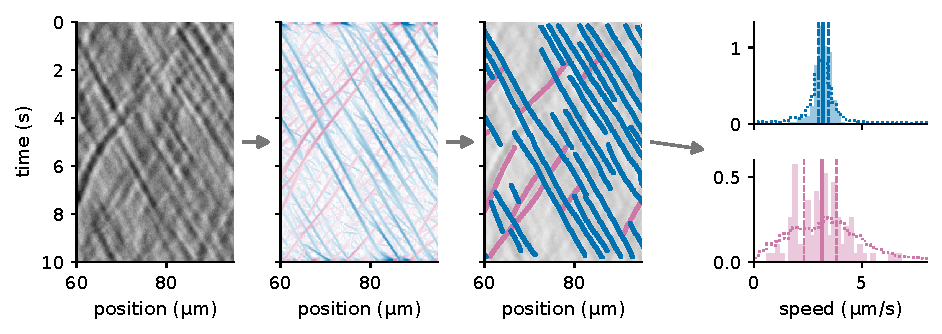
\includegraphics[width=\textwidth]{suppfig/FigS_streak_pipeline.pdf}
\caption{\textbf{Method for extracting directional speeds from kymographs.}
\textbf{(A)} TODO.
\textbf{(B)} TODO.
}
\label{fig:speed_flux_extraction_real_data}
\end{figure}

\clearpage

% -----------------------------------------------------------------------
% FIGURE: positions of all flow videos
% Actively referenced in main text (Results, "about 1500 flow videos"):
%   "SI Fig.~\ref{fig:video_positions}"
% Content: every filmed session's network with all video positions.
% Generated by transport_paper Working_notebooks/manuscript_figures/figS_video_positions.py
% -----------------------------------------------------------------------
\begin{figure}[hbt!]
\centering
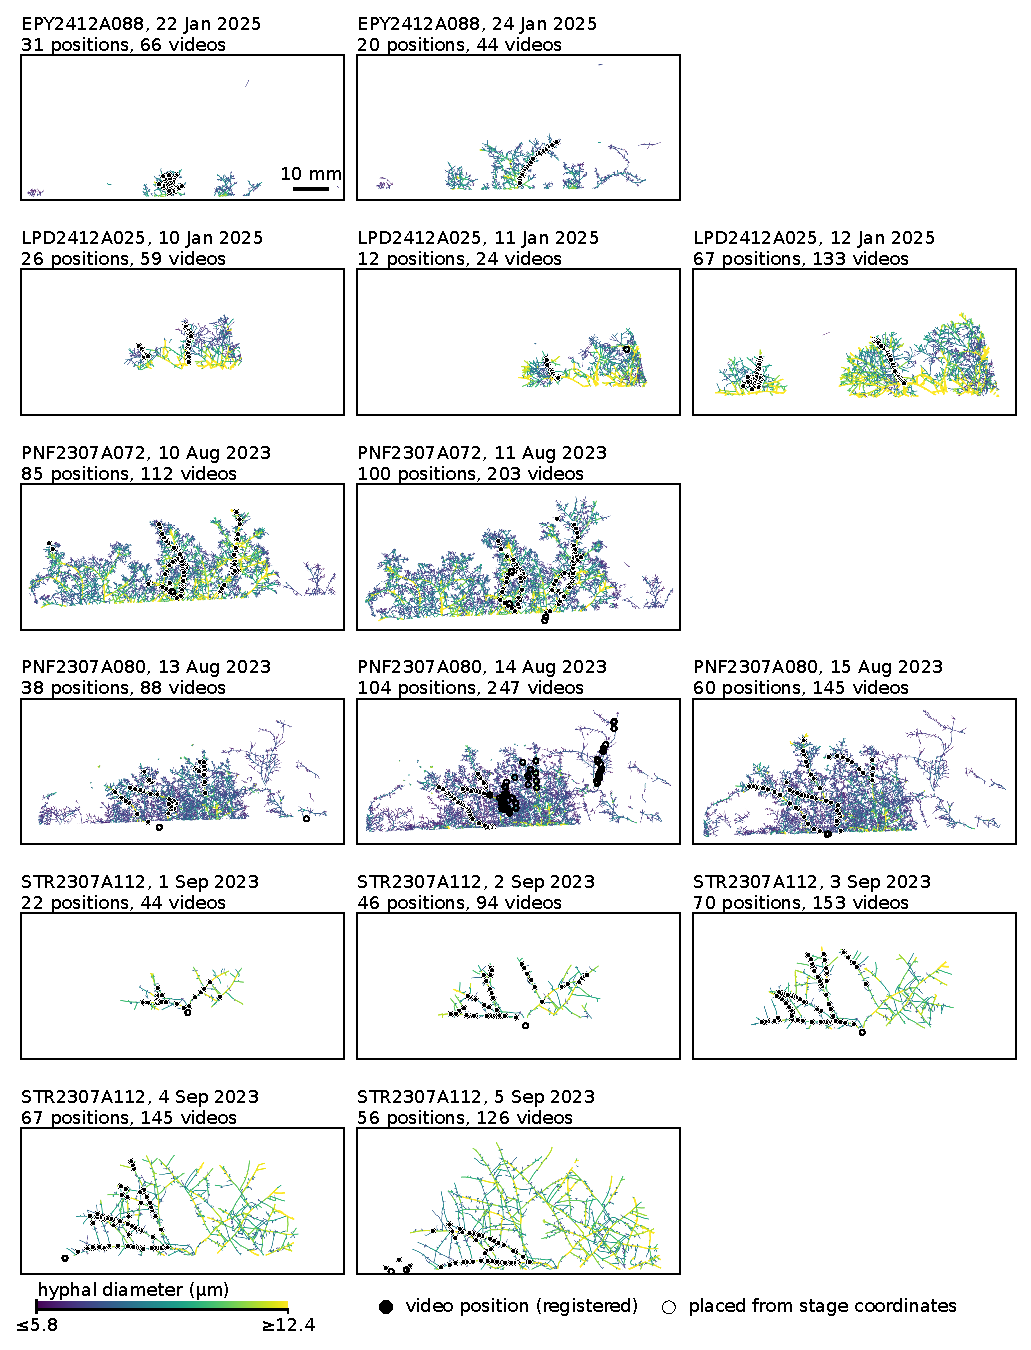
\includegraphics[width=\textwidth,height=0.85\textheight,keepaspectratio]{suppfig/FigS_video_positions.pdf}
\caption{\textbf{Positions of all flow videos.}
Each panel shows the network of one filmed session (5 colonies, 15 sessions, in time order per colony), drawn as in Fig.~\ref{fig:hyphal_profiling}A,B: colour indicates hyphal diameter.
Dots mark the 804 stage positions at which the 1,683 videos were taken (a bright-field video, mostly followed by a Nile Red video at the same position).
Filled dots are placed at the hyphae their videos were registered to; open dots (74 positions without a registered video) are placed from the microscope stage coordinates.
The LPD2412A025 sessions (10--12 Jan 2025) are days 10--12 of Fig.~\ref{fig:hyphal_profiling}B. All panels share the 10~mm scale bar.}
\label{fig:video_positions}
\end{figure}

\namedsubsection{Lid-on and lid-off flow videos}{subsec:si_lid}
% NOTE (10 Oct): section text to be written by Simon; cited from the main text (peristaltic streaming, flow reversals). Facts from transport_paper#121 (Simon, 2 Oct: a stated condition of the flow videos, Methods supplement):
% NOTE (1): sessions filmed with the lid off, before late 2023, show back-and-forth flow driven by air flow over the plate (docs log 2026-10-01-a-lid-off-dropbox-4x-session-showed-the-motion-gate-passing-drifting-static-texture.md).
% NOTE (2): the paper's sessions were filmed with the lid on; still to confirm for all sessions (Methods \todo at the flow-video paragraph).
% NOTE (3, open before writing): which sessions/plates were lid off and whether any enter the paper's tables; Snellius jobs 27439881 and 27439919 (2023 lid-off videos: curvature, synchronous swings, resolution) not yet read.

\namedsubsection{Size of the isolated segment}{subsec:si_segment_size}
% NOTE (10 Oct): section text to be written by Simon; cited from the main text (section cuts, "does not require the long range connectivity"). Facts from docs log 2026-09-29-registering-the-cut-videos-shows-the-stage-coordinates-are-off-by-millimetres-and-the-smallest-isolated-piece-loses-the-most-flow.md; analysis transport_paper Working_notebooks/figure3/section_cut_registered.py (branch feat/section-cut-registered 4a34453), outputs fig_outputs/perturbations/section_cut_registered/videos.csv.
% NOTE (1, data): cut-day videos registered by hand (Simon) onto arc-unit STG stores anchored on the last frame before the cut: LPD2412A025_t77, EPY2412A104_t82, EPY2412A084_t73, LPD2412A009_t90. LPD2412A023 cannot be registered (its segmented frames miss the long hyphae around the cut site).
% NOTE (2, piece size from the network): a piece is isolated when the cut splits it off its component (cut mark severs every edge within max(50 um, 2.5 map px)). Stores have segmentation gaps, so the 24 and 73 mm pieces may still be joined in reality.
% NOTE (3, post/pre speed on the same STG edges, 0-30 min / later): EPY2412A104, inside a 4.6 mm piece between two cuts (hand value 4.3 mm): 0.74 / 0.18 at 35-68 min; LPD2412A025, 24 mm piece, 1.4 mm from the cut: 0.26 / 0.68 at 80-326 min; EPY2412A084, 73 mm piece, 3 mm away: 0.78 / 0.84 at 30-58 min; LPD2412A009, still connected, 1.9 mm along the network: 0.80 / 0.66 at 93-119 min; at a cut stub (EPY104, LPD009): 0.10-0.50 / ~0.10.
% NOTE (4, reading in the log): the smallest isolated piece loses the most flow over time; whether the size dependence holds needs more than one small piece. Flow did not stop in any piece (main text), but at cut stubs it fell to ~0.1 of the pre-cut speed.
% NOTE (5, caveats): stage coordinates are unreliable on every cut plate (positions off by 0.2-2.3 mm; videos placed by frame matching and Coco's map labels instead); registrations give the edge, not the position along it; EPY104 videos 22 and 28 may sit outside the piece (Coco's labels vs registration). The writeup science/section_cut_sites.typ (rhizosphere PR #240) still carries the older stage-position numbers.

\namedsubsection{Selection bias of the filmed hyphae}{subsec:si_video_selection}
% NOTE (10 Oct): section text to be written by Simon; the facts (definition, numbers, caveats) are in the note above the figure below.
% NOTE (10 Oct, outline for this section, facts only; sources: transport_paper feat/bc-selection-bias d2054b7, manuscript/bc_selection_bias.md, #130):
% NOTE (1, why): the flow videos were taken by eye on runner hyphae where the two streams could be told apart (main text, Results opening). Speed statistics therefore describe the filmed hyphae, not the network as a whole; this section measures how different the filmed edges are, so the reader can judge how far the results generalise.
% NOTE (2, measure): betweenness centrality (BC) as defined by Oyarte Galvez et al. 2025 (oyarte_galvez_travelling-wave_2025, after freeman_set_1977): for each edge, the number of shortest paths (by edge length; equal-length paths share 1/sigma each) from every node of the session network to the root compartment, i.e. one super-node joined at zero length to all annotated roots; divided by the number of source nodes, so it is the share of nodes whose route to the root crosses the edge. Edges with BC = 0 are left out (62,469 of 1,139,071; 42 filmed). Variant: sources = growing tips only.
% NOTE (3, groups): filmed edges = store edges that carry a video mapping (1,972 with BC > 0, 15 sessions on 5 plates). References: all edges of the same session networks (1,076,602), and, to separate selection from where the plates were filmed, the edges inside the convex hull of the filmed positions (310,967).
% NOTE (4, result): filmed edges sit at a median 82nd percentile of BC within their own network (IQR 54-95); every session's median is above 50 (73-96; Wilcoxon over sessions p = 6e-5). Median log10 BC: filmed -2.40, all -3.80, inside the hull -3.83, so the shift is selection, not spatial extent. Per session, P(filmed > other edges) 0.63-0.89. Tips-only BC gives the same picture: 80th percentile (IQR 61-92), session medians 64-95; rank correlation of the two BC variants across edges 0.78.
% NOTE (5, what else differs): filmed edges are thicker (store diameter 10.0 vs 7.8 um), slightly closer to a growing tip (4.3 vs 4.8 mm), and far less often tree-like (15 % vs 36 %; 33 % inside the hull). BC and diameter covary, so the diameter difference is not a separate selection.
% NOTE (6, consequence for the speeds, panel C): among filmed edges, bright-field median speed rises weakly with log BC in both directions: Spearman 0.18 to tip (n 1,706) and 0.18 to root (n 1,555), unchanged with tip distance partialled out; positive in 12/15 and 14/15 sessions. Same direction as Oyarte Galvez (speeds in both directions rise with BC) but weak; tips-only BC gives 0.39 / 0.36 raw, 0.21 / 0.25 with tip distance partialled out.
% NOTE (7, caveats): edges along one hypha share nearly the same BC, so pooled p-values overstate independence (the per-network percentiles are the robust statistic); edges counted, not weighted by length (Oyarte's Extended Data Fig 7a is length-weighted); store diameters for both groups (no lumen diameters network-wide).

% -----------------------------------------------------------------------
% FIGURE: selection bias of the filmed hyphae, root-directed betweenness centrality
% Generated by transport_paper Working_notebooks/manuscript_figures/figS_bc_selection.py (d2054b7, branch feat/bc-selection-bias; transport_paper#130)
% NOTE (9 Oct, caption is Simon's to write; facts): BC as in Oyarte Galvez 2025: for every edge, the number of shortest paths
% (by edge length; ties split 1/sigma) from every node of the session network to the root compartment (one super-node joined to
% all annotated roots), divided by the number of source nodes; edges with BC = 0 dropped. Variant: sources = growing tips only.
% Filmed edges = store edges carrying a video mapping (1,972 with BC > 0, 15 sessions); reference = all 1,076,602 edges, and the
% 310,967 inside the convex hull of the filmed positions. (A) log10 BC: median -3.80 all, -3.83 in hull, -2.40 filmed;
% P(filmed > rest) 0.75. (B) percentile of the filmed edges within their own network: median 82 (IQR 54-95), session medians
% 73-96, all above 50; tips-only variant 80 (61-92), session medians 64-95. (C) bright-field median speed per filmed edge vs log
% BC: Spearman 0.18 to tip (n 1,706) and 0.18 to root (n 1,555), unchanged with tip distance partialled out; positive in 12/15
% and 14/15 sessions (Oyarte: both speeds rise with BC). Filmed edges also: store diameter 10.0 vs 7.8 um, tip distance 4.3 vs
% 4.8 mm, tree-like 15 % vs 36 % (33 % in hull). Caveats: edges of one hypha share BC, so pooled p-values are anti-conservative
% (use the percentiles); edge counts not length-weighted; store diameters for both groups.
% -----------------------------------------------------------------------
\begin{figure}[hbt!]
\centering
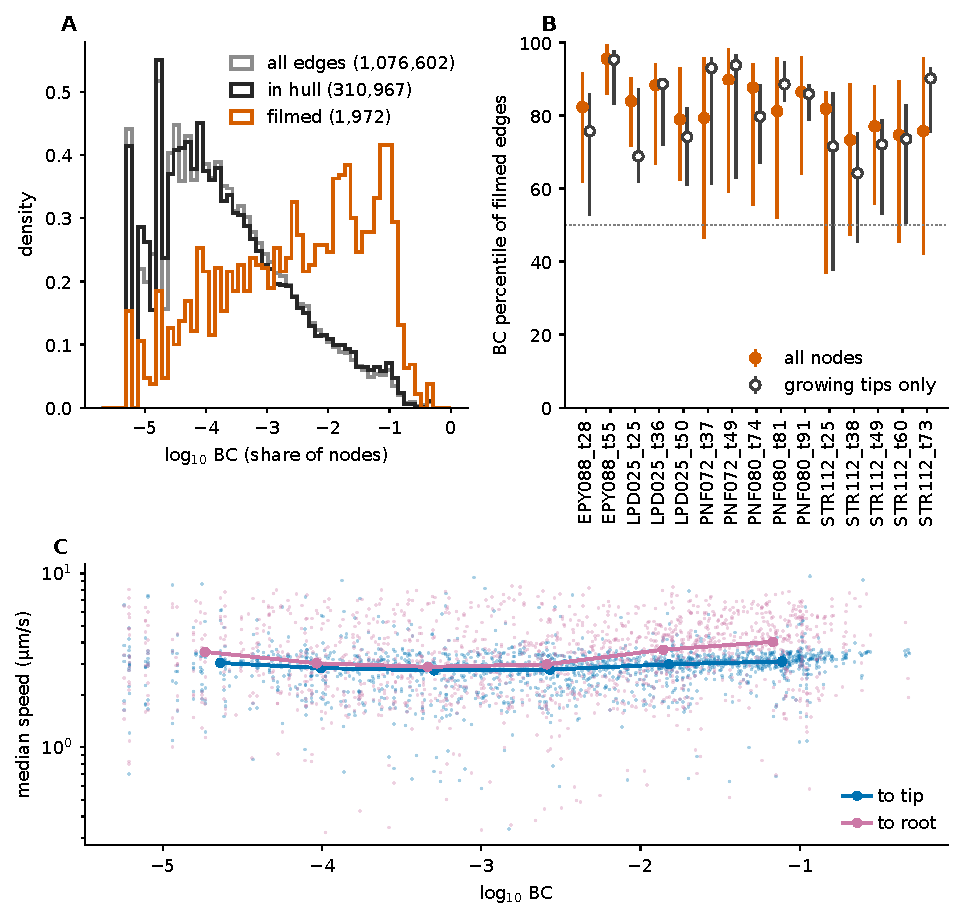
\includegraphics[width=\textwidth,keepaspectratio]{suppfig/figS_bc_selection.pdf}
\caption{[Caption to be written.]}
\label{fig:bc_selection}
\end{figure}

\namedsubsection{Tree-like edges and distance to the growing tips}{subsec:si_tree_tip}
% NOTE (10 Oct): section text to be written by Simon; cited from the Fig 1A caption (inset). Facts (transport_paper master, Working_notebooks/manuscript_figures/fig1.py, bridge_share_by_tip(); recomputed 10 Oct):
% NOTE (1, definition): an edge is tree-like when it is a bridge of the network graph (removing it disconnects the network; networkx bridges on the simple graph, degree-2 nodes dissolved), as in the model tables' `bridge` column; otherwise it lies on a loop. Methods, \nameref{subsec:dated_graph}, paragraph "Tree and loop edges", has the definition and a \todo for these bins.
% NOTE (2, edges): the filmed edges of the main model tables, 15 sessions (loop_density_curve.prepare_edges): 1,590 edges, 1,579 with a tip distance; tip distance = network distance to the nearest growing tip (d_tip, model_accuracy/features_edges.csv).
% NOTE (3, numbers, bins by tip distance in mm, n edges / % tree-like): <1: 86 / 39.5 %; 1-2: 201 / 20.4 %; 2-4: 438 / 10.5 %; 4-8: 568 / 10.7 %; >8: 286 / 14.3 % (main text: 40 % within 1 mm vs 11-14 % beyond 2 mm).
% NOTE (4, context): over all edges of the same networks 36 % are tree-like vs 15 % of the filmed edges (\nameref{subsec:si_video_selection}), so the filmed set under-samples tree-like edges.
% NOTE (5, open): a figure (share by tip distance, filmed vs all edges) if wanted; per-session spread.

\namedsubsection{Movement at the growing tips}{subsec:si_tips}
% NOTE (10 Oct): section text to be written by Simon; to be filled with more data later (Simon: does not lead to many conclusions yet). Sources: transport_paper explore/tip-diffusion (f4a8ba7, 37c25b3), manuscript/tip_diffusion_sketch.md; AMF_Transport#5; transport_paper#132 Q1.
% NOTE (1, streaks vs tip distance, bright-field, 654,711 streaks, 15 sessions): median to-tip streak duration 1.20 s within 0.5 mm of a tip vs 1.40-1.45 s beyond 1 mm; length 2.6 vs 4.2-4.5 um (shorter because slower, not shorter-lived). Per kymograph: median 38 moving streaks within 0.5 mm vs 118-149 beyond 2 mm; no moving streak in 20 % of kymographs within 1 mm vs 5-8 % beyond; static share of streaks 0.31 vs 0.02-0.04. Structure-tensor coherence flat (0.74-0.79). Many near-tip kymographs look clean but low-SNR (Simon). Caveats: detector minimum 15 frames (0.75 s) censors short or irregular movement; tip edges are short and counts are not length-normalised; streaks pooled without bootstrap.
% NOTE (2, videos with a tip in frame): the filmed positions rarely include a tip (selection, \nameref{subsec:si_video_selection}). In the first frames of the 96 videos nearest a tip (graph tip distance < 1.5 mm), 5 bright-field 20 fps videos have a free tip in frame (8 tip branches; STR2307A112, EPY2412A088, LPD2412A025, PNF2307A080, PNF2307A072); 2 more are 0.5 / 0.1 fps time-lapses.
% NOTE (3, kymographs traced by hand from the apex, figure below): within ~20 um of the apex movement is sparse and slow (~0.5-1 um/s, read by eye), in both directions in some branches, with stalls, small steps back and oscillations (period ~2 s, no net motion); much of the last 20 um is static; no long straight ~3 um/s streaks as elsewhere in the network. Low SNR; one video's apex uncertain.
% NOTE (4, open): more tip videos (targeted recordings, or a scan of the other video sets); particle tracking for an MSD; link to the near-tip slowdown (Fig 1E) and to the main-text qualifier 'no sign of random or back-and-forth movement'.

% -----------------------------------------------------------------------
% FIGURE: kymographs along tip branches, traced by hand from the apex
% Generated by transport_paper Working_notebooks/tip_crops_snellius.py (on Snellius) + tip_kymos_handtraced.py (explore/tip-diffusion 37c25b3)
% NOTE (10 Oct, caption is Simon's to write; facts): one row per tip branch; left: first frame with the trace (red) and the apex (cyan);
% middle: raw kymograph (x = distance from the apex along the hypha, um; y = time, s), mean over +/-3 px across the hypha;
% right: same with the time-mean removed (moving features only). 0.069 um/px, 20 fps; 10 s videos except PNF2307A072 (30 s).
% Rows: STR2307A112 2023-09-04 13:04:46 short and long branch; EPY2412A088 2025-01-22 12:12:01 branches a, b (trace off the hypha
% beyond ~15 um in b); LPD2412A025 2025-01-12 18:27:52 curled and right branch; PNF2307A080 2023-08-13 21:42:19; PNF2307A072
% 2023-08-10 14:35:58 (apex uncertain).
% -----------------------------------------------------------------------
\begin{figure}[hbt!]
\centering
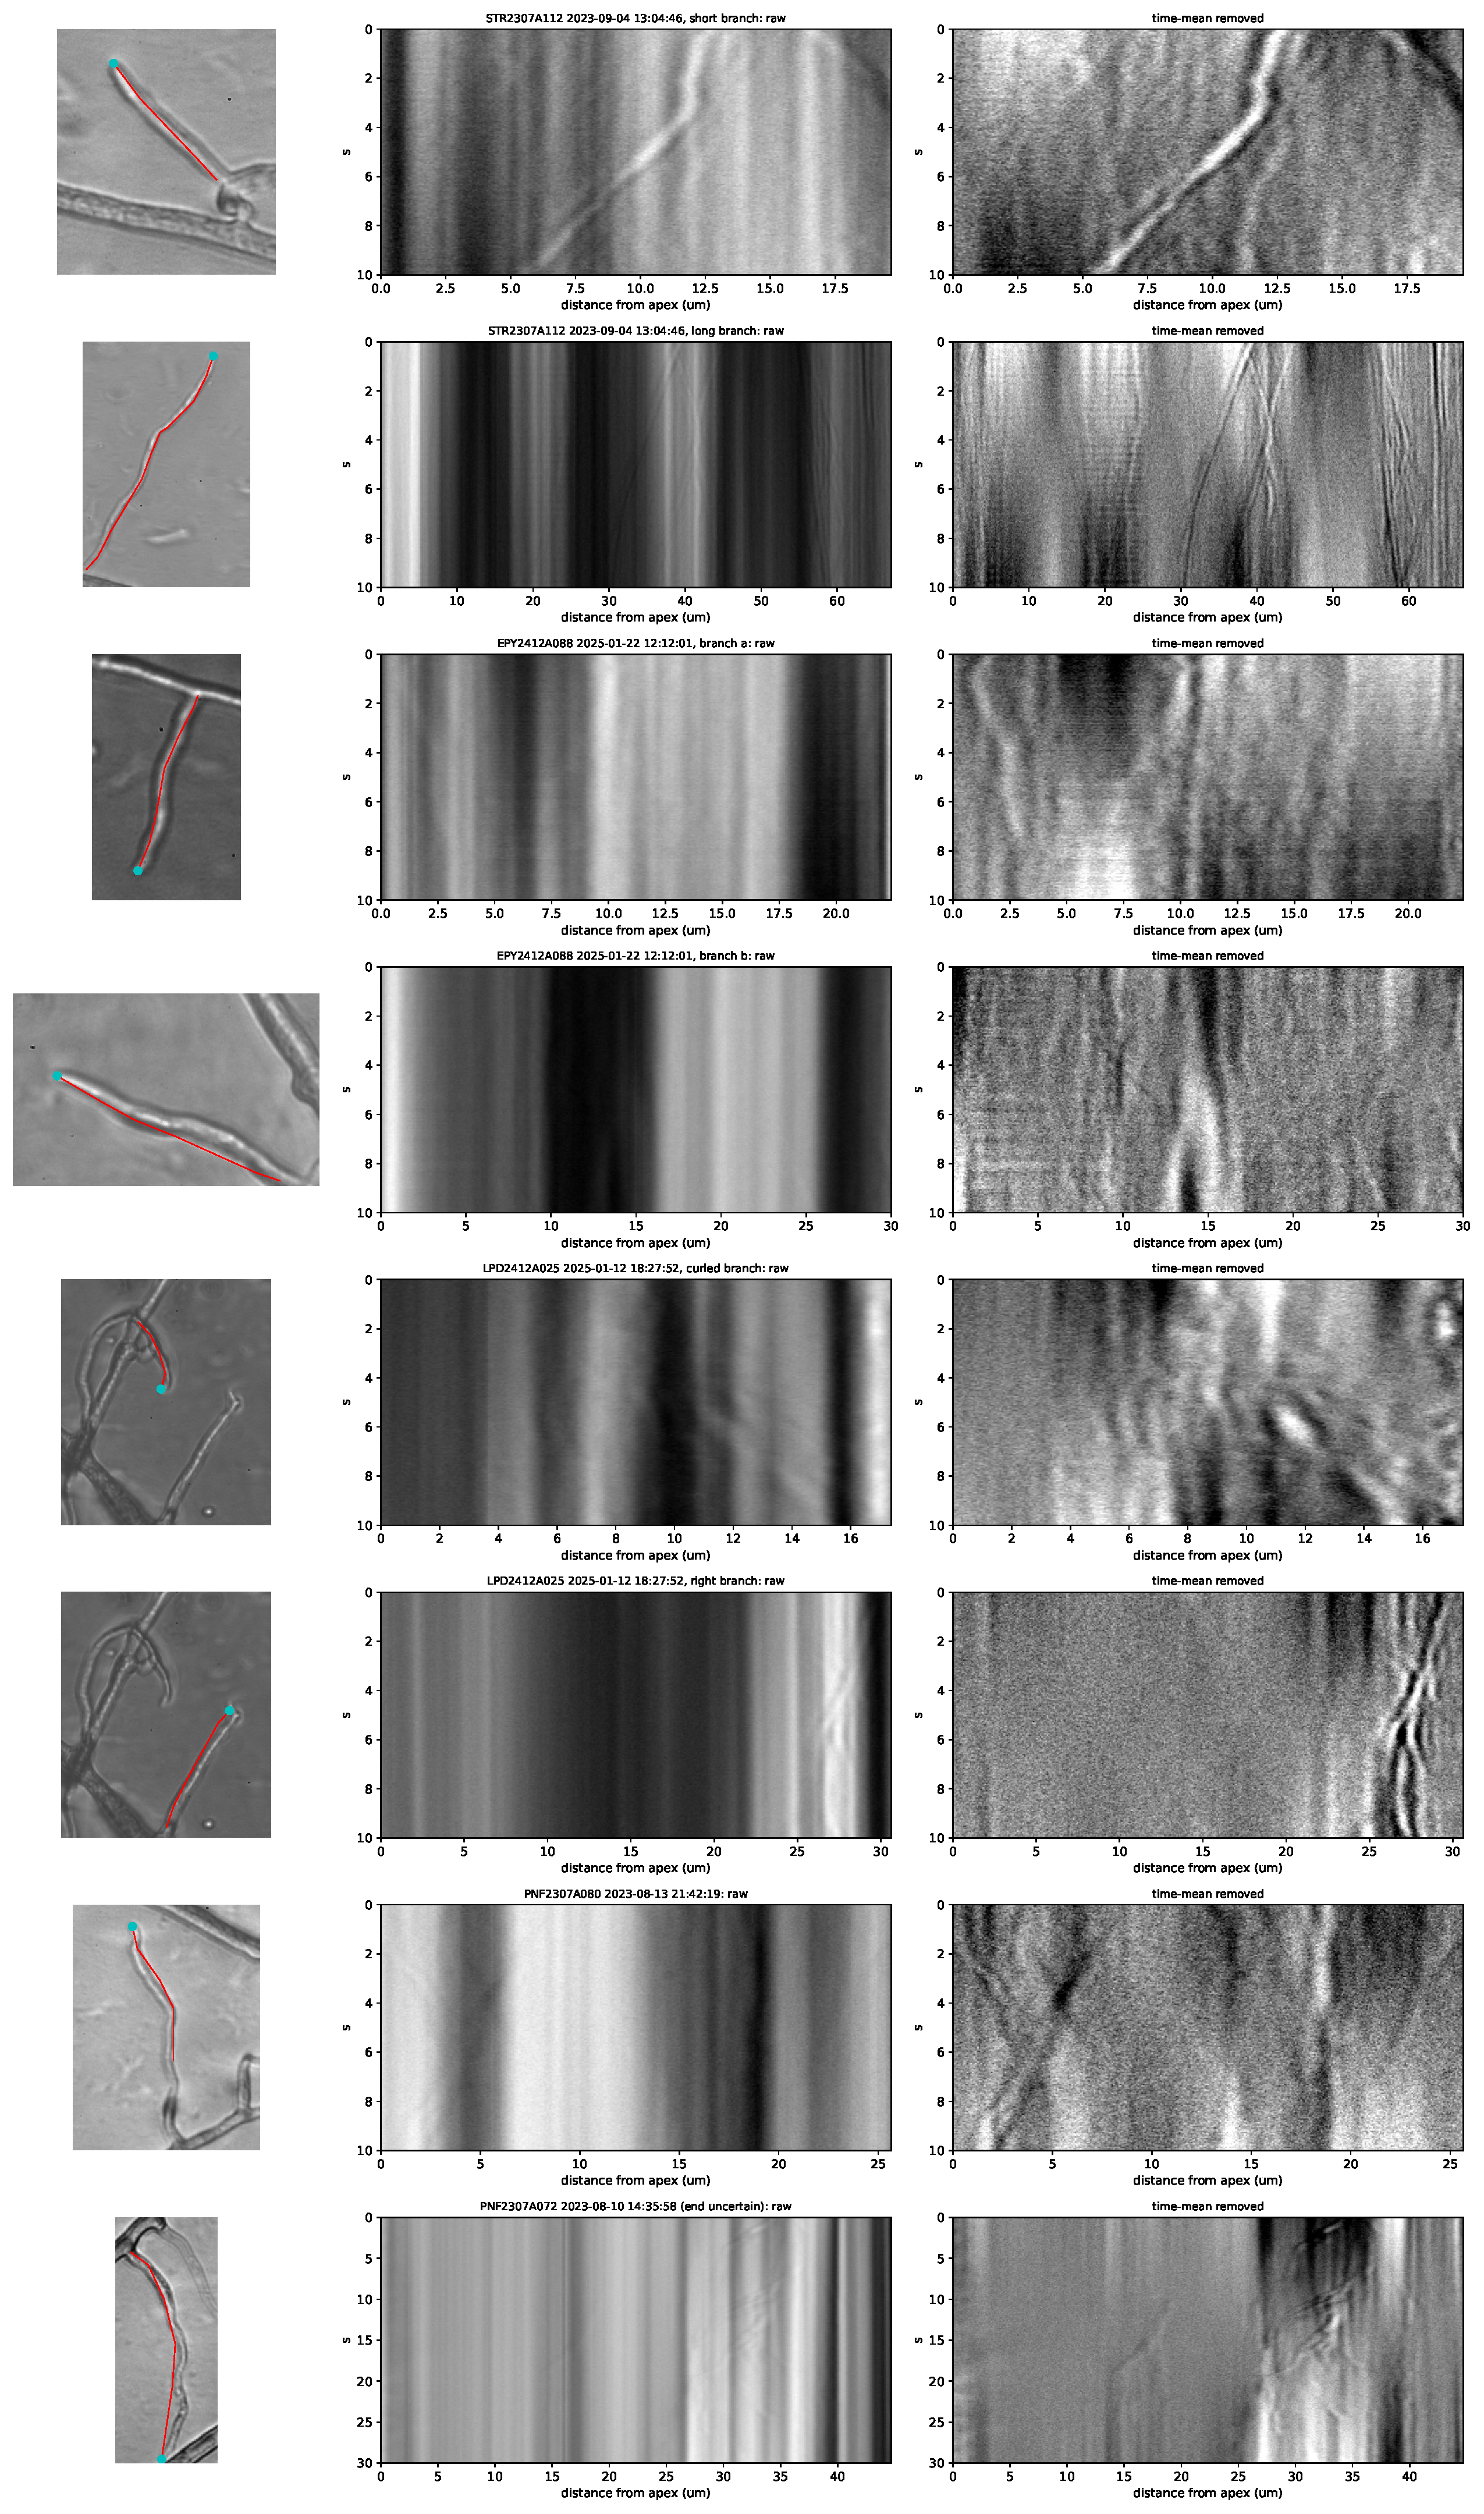
\includegraphics[width=\textwidth,height=0.9\textheight,keepaspectratio]{suppfig/figS_tip_kymos.pdf}
\caption{[Caption to be written.]}
\label{fig:tip_kymos}
\end{figure}

% -----------------------------------------------------------------------
% FIGURE: spread (IQR) of the speeds of all static-flow videos
% Referenced in main text (Results): "SI Fig.~\ref{fig:speed_iqr}"
% Generated by transport_paper Working_notebooks/manuscript_figures/figS_video_positions.py
% -----------------------------------------------------------------------
\begin{figure}[hbt!]
\centering
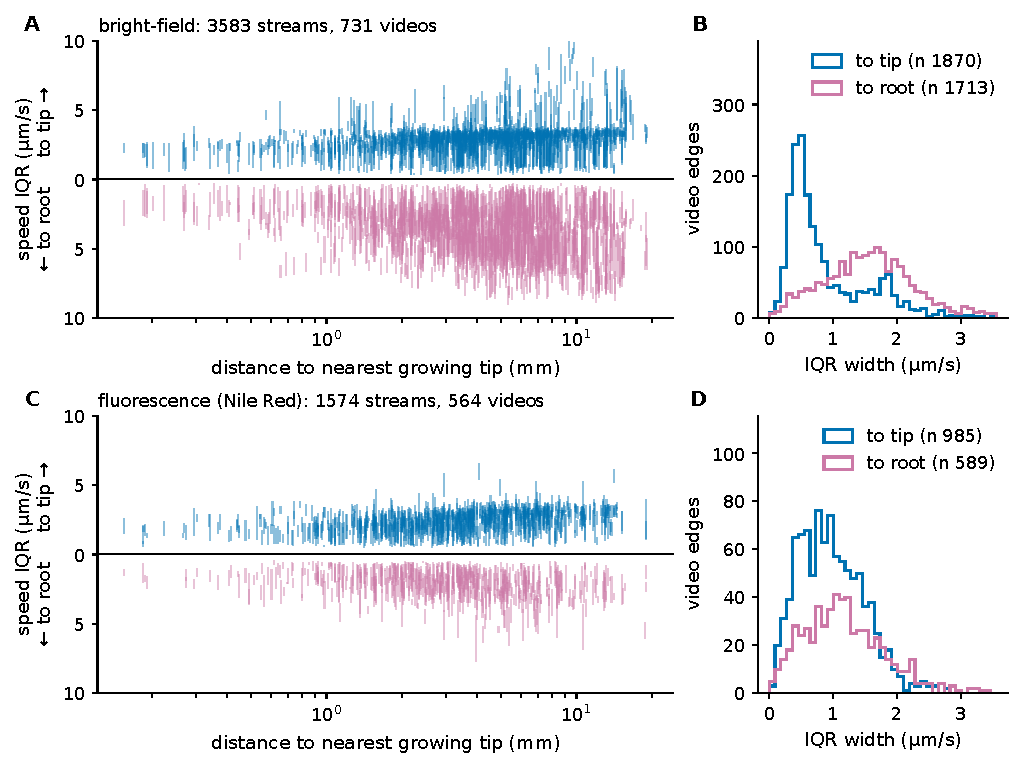
\includegraphics[width=\textwidth,keepaspectratio]{suppfig/FigS_video_positions_iqr.pdf}
\caption{\textbf{Spread of the speeds in the static-flow videos.}
Interquartile range (q25--q75) of the extracted to-tip and to-root speeds of each filmed hypha in the bright-field videos (3,583 hypha-direction streams from 731 videos; root-cut, section-cut and salt-shock videos excluded; directions with fewer than 5 streaks omitted).
Streaks count when they span at least 15 frames in bright-field (20~fps) and at least 5 frames in fluorescence (1--2~fps).
\textbf{(A, B)} Bright-field.
\textbf{(C, D)} Fluorescence (Nile Red) videos, same rules and axis ranges (2,385 streams from 625 videos).
\textbf{(A, C)} Bars against distance to the nearest growing tip, to-tip up (blue) and to-root down (pink).
\textbf{(B, D)} Distribution of the IQR widths.
The median IQR is 0.63~$\mu$m/s to tip and 1.58~$\mu$m/s to root in bright-field, and 1.07~$\mu$m/s to tip and 1.22~$\mu$m/s to root in fluorescence.}
\label{fig:speed_iqr}
\end{figure}
% NOTE (10 Oct, IQRs of censored speeds (transport_paper#132 comment 6088415445; feat/fl-numbers-limits 8391a7e, manuscript/fl_numbers_limits.md)): median IQR to tip / to root, streaks < 5 um/s in both modes: bright-field 0.62 / 1.25, Nile Red 1.06 / 1.17 (directions with q75 < 5: 0.60 / 1.41 vs 1.07 / 1.18). So the bright-field to-root spread drops toward Nile Red once truncated, the to-tip one does not. Nile Red directions have a median of 14 streaks vs 87 in bright-field.

% -----------------------------------------------------------------------
% FIGURE: to-tip against to-root speed per edge, fluorescence vs bright-field
% Same plot as Fig.~\ref{fig:asymmetries}A (fig2.py, draw_arm_density), fed with the
% fluorescence data. Numbers from the min_frames=5 fluorescence streaks (7 Oct).
% Generated by transport_paper Working_notebooks/manuscript_figures/figS_video_positions.py
% -----------------------------------------------------------------------
\begin{figure}[hbt!]
\centering
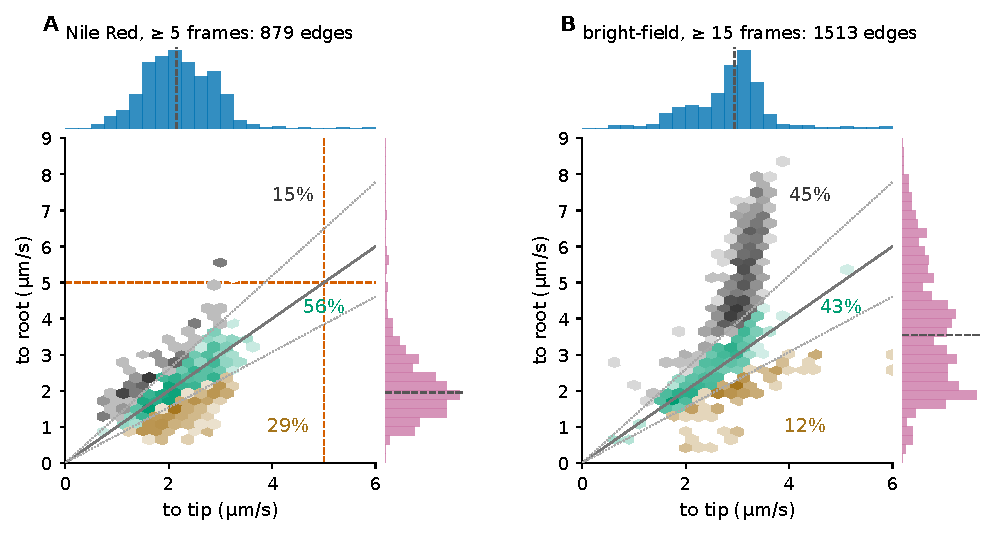
\includegraphics[width=\textwidth,keepaspectratio]{suppfig/figS_fl_forward_backward_density.pdf}
\caption{\textbf{To-tip against to-root speeds in fluorescence and bright-field.}
Density plots of the absolute to-tip speed against the absolute to-root speed at the same location, drawn as in Fig.~\ref{fig:asymmetries}A, for \textbf{(A)} the Nile Red fluorescence videos and \textbf{(B)} the bright-field videos (static-flow videos only; streaks of at least 5 frames in fluorescence and 15 frames in bright-field; 879 fluorescence and 1,513 bright-field edges with both directions, as given above each panel).
Median speeds are 2.15~$\mu$m/s to tip and 1.96~$\mu$m/s to root in fluorescence, against 2.95 and 3.55~$\mu$m/s in bright-field.
Marginal histograms with medians (dashed); hexes are coloured by their relation to 1:1 within a factor 1.3 (to-root faster, similar, to-tip faster) with the share of edges in each category.
Fluorescence videos were imaged at 1 or 2~fps (10 or 20 frames) against 20~fps for bright-field.
The dashed lines in A at 5~$\mu$m/s mark a rough estimate of where under-sampling could start, assuming a feature spacing of about 5~$\mu$m in the Nile Red kymographs (2.5~$\mu$m per frame at 2~fps); this spacing was not measured.}
\label{fig:fl_forward_backward}
\end{figure}
% NOTE (10 Oct (transport_paper#132 comment 6088415445; feat/fl-numbers-limits 8391a7e, manuscript/fl_numbers_limits.md)): caption medians 2.15 / 1.96 vs 2.95 / 3.55 are full-range streak medians (Nile Red censored above ~5). Per-pixel (2 fps, >= 100 px): Nile Red 2.42 / 2.20 (595 edges) vs bright-field 2.74 / 2.91 (1,513); paired 532 edges 2.38 / 2.15 vs 2.56 / 2.46. The dashed 5 um/s line stands, but its rationale ('rough estimate, feature spacing') is superseded: the limit is measured (half-peak 4.9 um/s at 2 fps, 4.7-5.1 at 1 fps; fig:fl_detection_limit).

% -----------------------------------------------------------------------
% FIGURE: detection of fluorescence streaks against speed
% Referenced in Methods (subsec:fl_detection_limit): "SI Fig.~\ref{fig:fl_detection_limit}"
% Generated by transport_paper Working_notebooks/manuscript_figures/figS_fl_detection_limit.py
% Numbers: transport_paper fig_outputs/synthetic_streak_ceiling/ceilings.csv, bf_subsampled_fl/efficiency.csv,
% pixel_noise_control/speed_summary.csv (notes synthetic_streak_ceiling.md, bf_subsampled_fl_efficiency.md,
% pixel_noise_control.md, 7 Oct).
% -----------------------------------------------------------------------
\begin{figure}[hbt!]
\centering
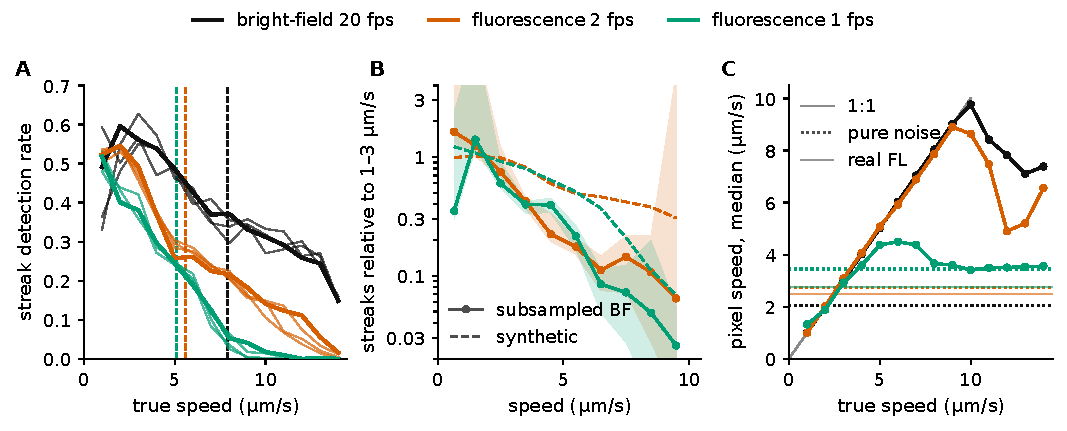
\includegraphics[width=\textwidth,keepaspectratio]{suppfig/figS_fl_detection_limit.pdf}
\caption{\textbf{Detection of fluorescence streaks against speed.}
Bright-field at 20~fps (black), fluorescence at 2~fps (orange) and at 1~fps (green), in all panels.
\textbf{(A)} Fraction of synthetic particles found as a streak against their true speed, for synthetic kymographs passed through the same normalisation, resampling, orientation filter and streak detection as the data (particles of 0.8~$\mu$m FWHM moving in both directions, calibrated density, automatic filter centre; streaks of at least 15 frames in bright-field and 5 in fluorescence).
Thick lines: exposure 0.9 of the frame period, as in the experiments; thin lines: exposure 0.01, 0.1 and 0.5, which coincide with it.
The detection rate falls to half its low-speed peak at 10.7~$\mu$m/s in bright-field, 4.9~$\mu$m/s at 2~fps and 4.7 to 5.1~$\mu$m/s at 1~fps (5 or 8 frames minimum).
Dashed vertical lines: 99th percentile of the measured streak speeds in each mode (7.9, 5.6 and 5.1~$\mu$m/s).
\textbf{(B)} Bright-field kymographs (1,296 kymographs, three plates) averaged and decimated to 2 and 1~fps and run through the fluorescence settings: streaks found per bright-field streak in the same 1~$\mu$m/s speed bin, relative to the mean of the 1 to 3~$\mu$m/s bins (solid, with the plate-then-kymograph bootstrap 95\% interval, cut at the axis limits; bins with fewer than 100 bright-field streaks omitted; logarithmic axis).
At 5 to 6~$\mu$m/s this is 0.18 at 2~fps and 0.22 at 1~fps (0.050 and 0.030 streaks per bright-field streak), against 0.49 and 0.51 for the synthetic efficiency of A at the same bins (dashed).
\textbf{(C)} Speed returned by the orientation filter per pixel, as the median over kymographs of the per-direction pixel median, against the true speed of synthetic particles moving in one direction at the calibrated density; grey line 1:1.
Dotted lines: the same statistic on pure-noise kymographs; thin solid lines: the median over the measured fluorescence directions.
At 2~fps the pixel median stays within 0.3~$\mu$m/s of the true speed up to 9~$\mu$m/s, at 1~fps it saturates at 4.4 to 4.5~$\mu$m/s (true speeds 5 to 7~$\mu$m/s) and falls back to the noise level from 8~$\mu$m/s.
The synthetic data are idealised: white pixel-independent noise, constant-speed Gaussian particles, no static structure or bleaching, and a weak calibration of density and noise, to which the limit in A is most sensitive.
In B the pipeline normalisation was applied to the 20~fps video before averaging and decimation, and the emulation was not checked against raw videos.}
\label{fig:fl_detection_limit}
\end{figure}
% NOTE (10 Oct (transport_paper#132 comment 6088415445; feat/fl-numbers-limits 8391a7e, manuscript/fl_numbers_limits.md)): the dashed 99th-percentile lines (7.9 / 5.6 / 5.1 um/s) come from the 8-frame production tables; for the 5-frame streaks the paper plots they are 8.1 (bright-field) / 6.1 (2 fps) / 5.3 (1 fps); figS_fl_detection_limit.py hard-codes the old values (same values in Methods L151). Caption C says pixel median valid 'up to 9 um/s', Methods says '8 to 9'.

% -----------------------------------------------------------------------
% FIGURE: to-tip against to-root speed per filmed hypha, coloured by distance to the nearest growing tip
% Generated by transport_paper Working_notebooks/manuscript_figures/figS_tip_root_scatter.py (161cf3f)
% NOTE (7 Oct, caption is Simon's to write; facts): one dot per video edge (one video of one hypha) with both streams
% measured, x/y = median absolute streak speed of each stream; colour = network distance to the nearest growing tip
% (mm, log scale 0.1-20, clipped; open grey = no tip distance); line = identity; axes cut at the 99.5th percentile (8 um/s).
% Same video edges, stream assignment and tip distance as the IQR figure (figS_video_positions); fluorescence = 5-frame
% streaks, bright-field = 15. (A) bright-field: 1,619 video edges (10 without tip distance), medians to tip 2.96 / to root
% 3.43 um/s, Spearman rho tip-root 0.64, to-root vs distance 0.25, to-tip vs distance 0.28. (B) Nile Red: 888 (6),
% 2.13 / 1.96 um/s, rho 0.53, 0.31, 0.29. Read: near tips the dots sit on the diagonal at ~2 um/s; both fast arms
% (to-root up to 8 um/s, and the horizontal fast to-tip arm at 4-8 um/s) are far from tips.
% NOTE (7 Oct, caveat for B, from the 'Fluorescence slow bias?' session, transport_paper#132): Nile Red streak speeds
% are censored above ~5 um/s (10-20 frames per video; half-peak ceiling 4.7-5.1 um/s vs 10.7 in bright-field). The
% absence of fast Nile Red dots in B is therefore not evidence that the fast streams carry no lipid; do not compare A and
% B above 5 um/s. Forward model: no evidence that the fast to-root stream is unstained, a twofold deficit not excluded.
% NOTE (7 Oct, later, SUPERSEDES the 'no evidence ... unstained' clause above; same session, transport_paper#132): per-pixel
% speeds (valid to ~8-9 um/s at 2 fps with >= ~100 pixels; not at 1 fps) show the detection limit explains only part of
% the smaller fast to-root branch in Nile Red. On 532 edges with both modes, to-root >1.3x faster on 39 % in bright-field
% vs 21 % in fluorescence (2 fps pixel medians 2.42 tip / 2.20 root um/s). Why less of the fast return is stained is open.
% -----------------------------------------------------------------------
\begin{figure}[hbt!]
\centering
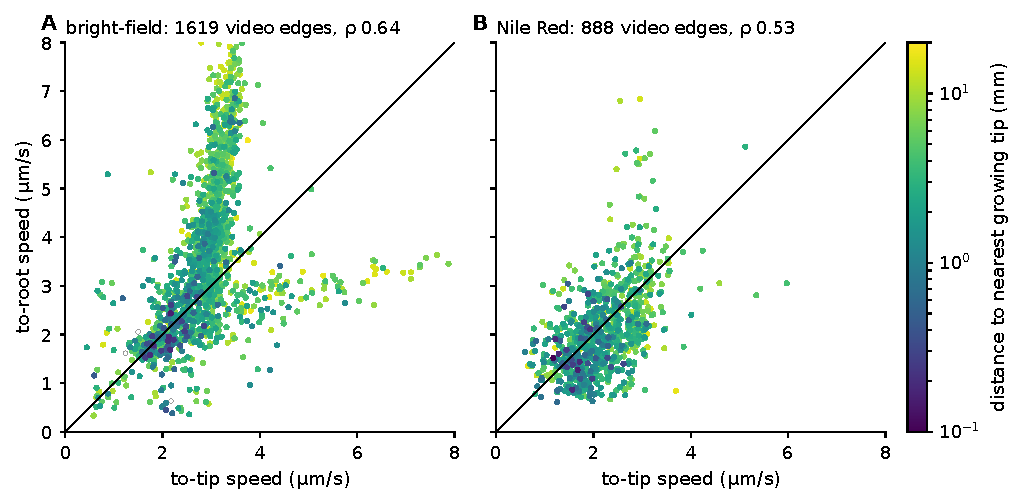
\includegraphics[width=\textwidth,keepaspectratio]{suppfig/figS_tip_root_scatter.pdf}
\caption{[Caption to be written.]}
\label{fig:tip_root_scatter}
\end{figure}
% NOTE (10 Oct, supersedes the Nile Red numbers in the note above (transport_paper#132 comment 6088415445; feat/fl-numbers-limits 8391a7e, manuscript/fl_numbers_limits.md)): panel B is streak medians, censored above ~5 um/s. Per-pixel at 2 fps: Nile Red 608 video edges, medians 2.40 / 2.20, rho 0.65; bright-field pixels 2,194 video edges, 2.76 / 2.73, rho 0.66.

% -----------------------------------------------------------------------
% FIGURE: osmotic shock, examples, response against osmolarity, Nile Red
% Referenced in main text (Results, osmotic paragraph): "SI Fig.~\ref{fig:salt_shock}D"
% Generated by transport_paper Working_notebooks/figure3/salt_shock_me.py (figS_salt_shock)
% -----------------------------------------------------------------------
\begin{figure}[hbt!]
\centering
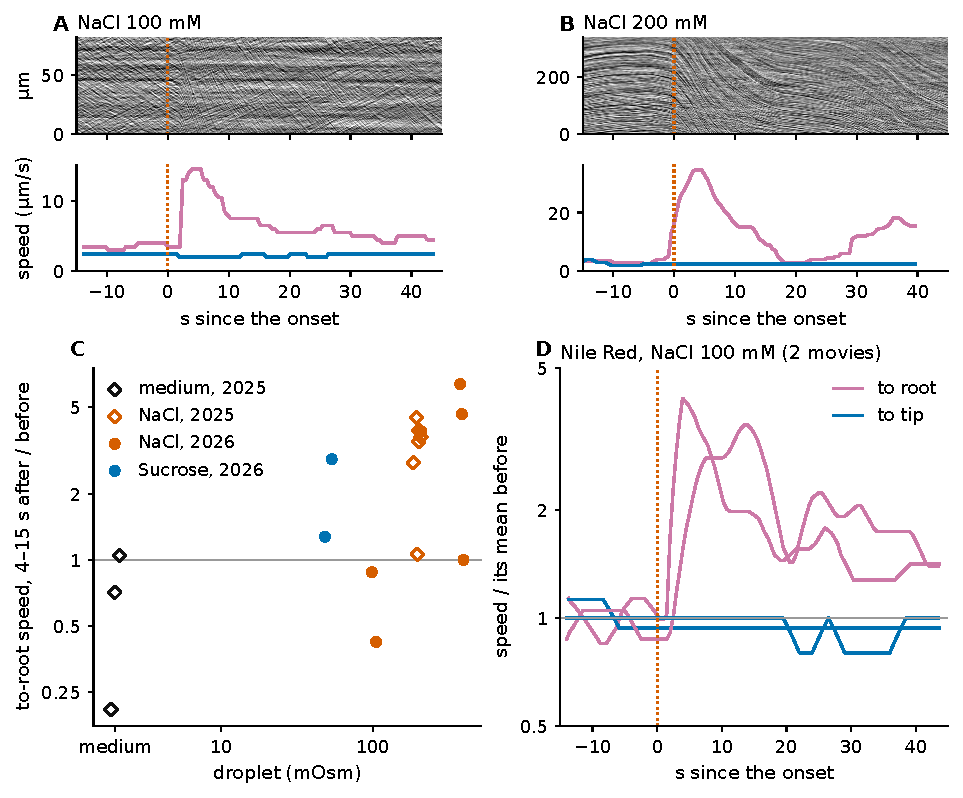
\includegraphics[width=0.9\textwidth,keepaspectratio]{suppfig/figS_salt_shock.pdf}
\caption{\textbf{Osmotic shock: examples, dependence on the droplet and lipid movement.}
\textbf{(A, B)} Two example kymographs after a drop of NaCl solution (100 mM and 200 mM) with the speed of the two streams below, to root (pink) and to tip (blue); dotted line: onset of the response.
\textbf{(C)} Change in the to-root speed, 4--15~s after the drop divided by $-10$ to $-1$~s before it, against the osmolarity of the droplet (medium-like drops at the left; NaCl in 2025 and 2026, sucrose in 2026).
\textbf{(D)} The two Nile Red fluorescence movies of NaCl 100 mM drops: speed to root (pink) and to tip (blue) divided by its mean before the drop.
The lipids, like the bright-field flow, keep their to-tip speed while the to-root speed rises.}
\label{fig:salt_shock}
\end{figure}

\clearpage

% -----------------------------------------------------------------------
% FIGURE S2
% Actively referenced in main text (lines 93, 97, 99, 144, 150):
%   "Fig. SI\ref{fig:carbonflow}b/d/e/f"
% Content: hydraulic (growth-induced mass-flow) model predictions vs
%          measurements; lipid volume-fraction spatial profile.
% Subfigures mentioned in text: b (predicted motor direction),
%   c (direction agreement, commented), d (speed comparison),
%   e (speed histogram), f (lipid volume fraction along hypha).
% -----------------------------------------------------------------------
\begin{figure}[hbt!]
\centering
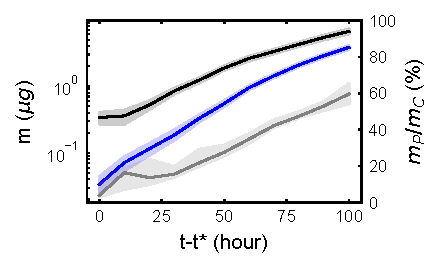
\includegraphics[width=\textwidth]{suppfig/FigS2.pdf} % WRONG FILE (checked 2 Oct): shows mass (ug) and m_P/m_C over t-t* (one panel), not the caption's 6 hydraulic panels. Candidate: transport_paper manuscript/figures/figS_net_flux.pdf (A: net lumen speed ~0.1-1 um/s, i.e. growth-driven flow alone is far below the measured 2-8 um/s); panels differ, caption needs rewriting.
\caption{\textbf{Growth-induced mass-flow model cannot explain observed speeds.}
\textbf{(A)} TODO.
\textbf{(B)} Predicted lipid flux direction from hydraulic minimisation.
Color indicates direction.
\textbf{(C)} Comparison of estimated and observed flux directions.
Percentage of agreement as a function of exclusion radius.
\textbf{(D)} Measured speed vs hydraulic model speed for all edges.
Model does not reproduce observed speeds.
\textbf{(E)} Histogram of absolute hydraulic speeds across whole network compared to measured bright-field speeds.
\textbf{(F)} Lipid volume fraction $\theta$ estimated from growth flux, plotted against distance from the hyphal tip.
}
\label{fig:carbonflow}
\end{figure}

\clearpage

% -----------------------------------------------------------------------
% FIGURE S3
% Referenced in commented-out text (line 64):
%   "SI Fig.\ref{fig:replicates}"
% Content: speed asymmetry dataset from 6 developmental time-points
%          across 2 plates, ~2000 edges total.
% Uncomment the section in main text (line 64) when this figure is ready.
% -----------------------------------------------------------------------
\begin{figure}[hbt!]
\centering
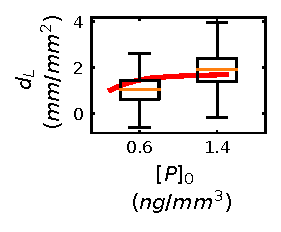
\includegraphics[width=\textwidth]{suppfig/FigS3.pdf} % WRONG FILE (checked 2 Oct): shows d_L against [P]_0 (boxplots), not speed asymmetry. No current replacement: needs a per-plate/per-session version of Fig 2A (to-root vs to-tip). figS_measurement_map.pdf shows where edges were measured, not the asymmetry.
\caption{\textbf{Speed asymmetry replicated across developmental time-points.}
\textbf{(A)} TODO: overview of all ~2000 measured edges across 6 time-points and 2 plates.
\textbf{(B)} TODO.
}
\label{fig:replicates}
\end{figure}

\clearpage

% -----------------------------------------------------------------------
% FIGURE S4
% Referenced in commented-out text (lines 83, 83):
%   "Figure \ref{fig:lipid_flows}d"  /  "SI Fig showing all replicates"
% Content: directional lipid kymographs and Fourier-filtered versions
%          showing net tipward flux; all replicate panels.
% Uncomment the section in main text (lines 82-84) when ready.
% -----------------------------------------------------------------------
\begin{figure}[hbt!]
\centering
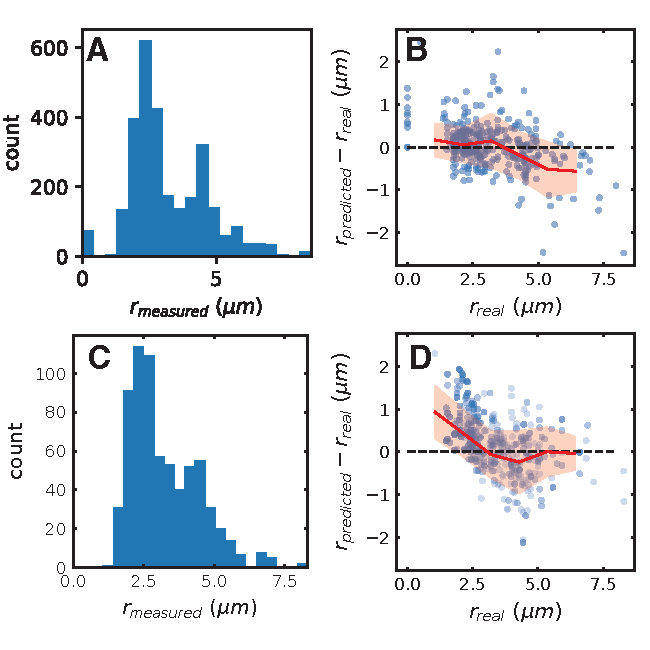
\includegraphics[width=\textwidth]{suppfig/FigS4.pdf} % WRONG FILE (checked 2 Oct): shows measured-radius histograms and r_predicted - r_real, not lipid direction. Closest: transport_paper manuscript/figures/figS_lipid_bias.pdf (per-plate share strongly to tip, fluorescence vs brightfield, vs tip distance); kymograph panels are already Fig 2D; caption needs rewriting.
\caption{\textbf{Lipid movement is predominantly tipward across all replicates.}
\textbf{(A)} TODO.
\textbf{(B)} TODO.
\textbf{(C)} TODO.
\textbf{(D)} Aggregate net flux direction in fluorescence (red) and bright-field (black) for all measured trails.
}
\label{fig:lipid_flows}
\end{figure}

\clearpage

% -----------------------------------------------------------------------
% FIGURE S5
% Referenced in commented-out text (line 165):
%   "Fig. \ref{fig:hydraulic_proportionality}b"
% Content: model prediction of C/P exchange proportionality emerging
%          from lipid-induced backflow.
% Uncomment the paragraph in main text (lines 164-167) when ready.
% -----------------------------------------------------------------------
\begin{figure}[hbt!]
\centering
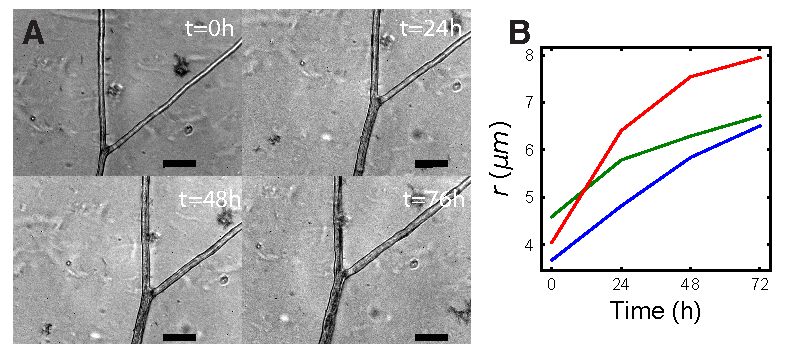
\includegraphics[width=\textwidth]{suppfig/FigS5.pdf} % WRONG FILE (checked 2 Oct): shows hyphae thickening over 72 h (images, r vs time), not C/P exchange. No current replacement in transport_paper.
\caption{\textbf{Lipid-backflow model predicts proportional C/P exchange.}
\textbf{(A)} TODO.
\textbf{(B)} Carbon flux from plant vs phosphorus flux from fungal colony under the backflow model, showing proportional scaling.
}
\label{fig:hydraulic_proportionality}
\end{figure}

\clearpage

% -----------------------------------------------------------------------
% ADDITIONAL FIGURES (not yet labelled in main text)
% Assign \label and add \ref in main text when ready to use.
% -----------------------------------------------------------------------

\begin{figure}[hbt!]
\centering
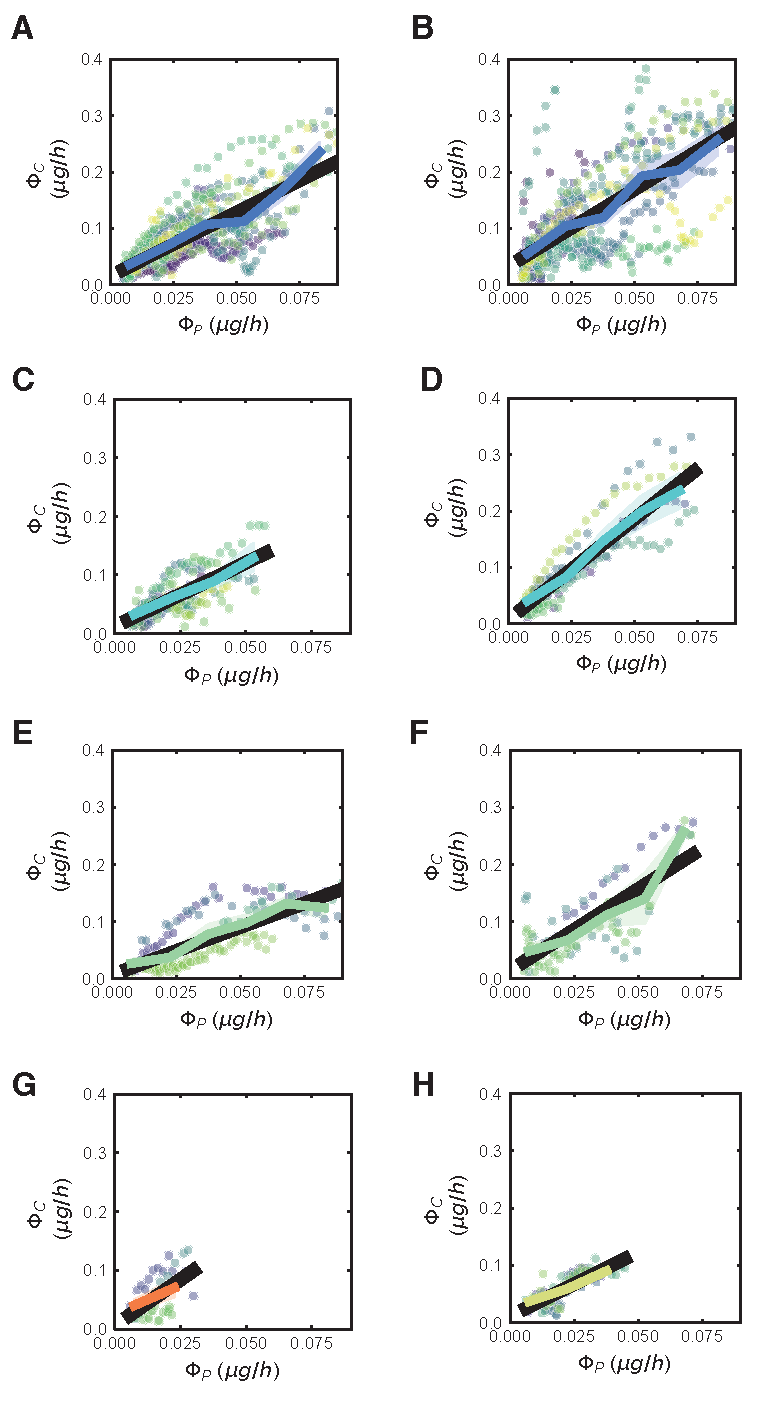
\includegraphics[width=\textwidth,height=0.8\textheight,keepaspectratio]{suppfig/FigS_replicate_4A.pdf}
% TRIAGED 2 Oct: Phi_C vs Phi_P (ug/h), 8 replicates A-H with linear fits: the C-P proportionality data (Bisot et al.). Goes with transport_paper#128 (C/P framing): keep if that framing stays, or cite if published.
\caption{\textbf{TODO: Replicate 4A.}
TODO caption.}
% \label{fig:replicate_4A}
\end{figure}

\clearpage

\begin{figure}[hbt!]
\centering
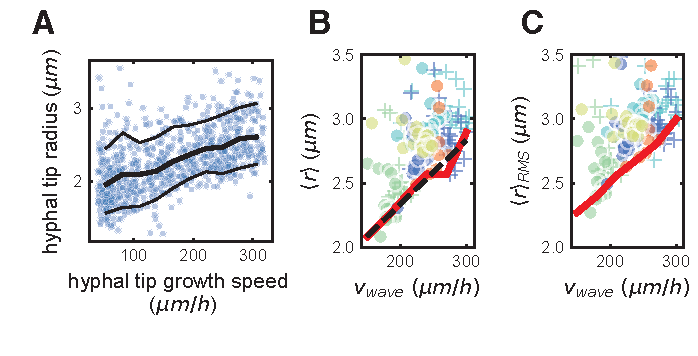
\includegraphics[width=\textwidth]{suppfig/FigSradius_speed.pdf}
% TRIAGED 2 Oct: tip radius vs tip growth speed, <r> vs travelling-wave speed: from the travelling-wave work (Oyarte Galvez 2025), not transport. Suggest drop unless a width-speed argument needs it (transport_paper#129).
\caption{\textbf{TODO: Radius vs speed.}
TODO caption.}
% \label{fig:radius_speed}
\end{figure}

\clearpage

\begin{figure}[hbt!]
\centering
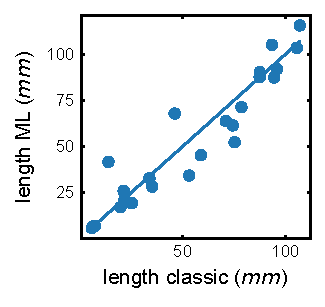
\includegraphics[width=\textwidth]{suppfig/FigureComparison.pdf}
% TRIAGED 2 Oct: network length, ML vs classic segmentation (~25 points): an older segmentation check. Suggest replace with transport_paper manuscript/figures/S_segmenter.png (current pipeline) or drop (transport_paper#129).
\caption{\textbf{TODO: Comparison figure.}
TODO caption.}
% \label{fig:comparison}
\end{figure}

\clearpage

\begin{figure}[hbt!]
\centering
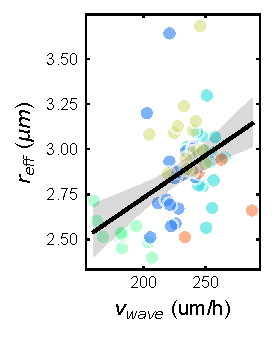
\includegraphics[width=\textwidth]{suppfig/FigureSRspeeddrag.pdf}
% TRIAGED 2 Oct: r_eff vs travelling-wave speed: travelling-wave work, not transport. Suggest drop (transport_paper#129).
\caption{\textbf{TODO: Speed-drag figure.}
TODO caption.}
% \label{fig:speed_drag}
\end{figure}

\clearpage

\begin{figure}[hbt!]
\centering
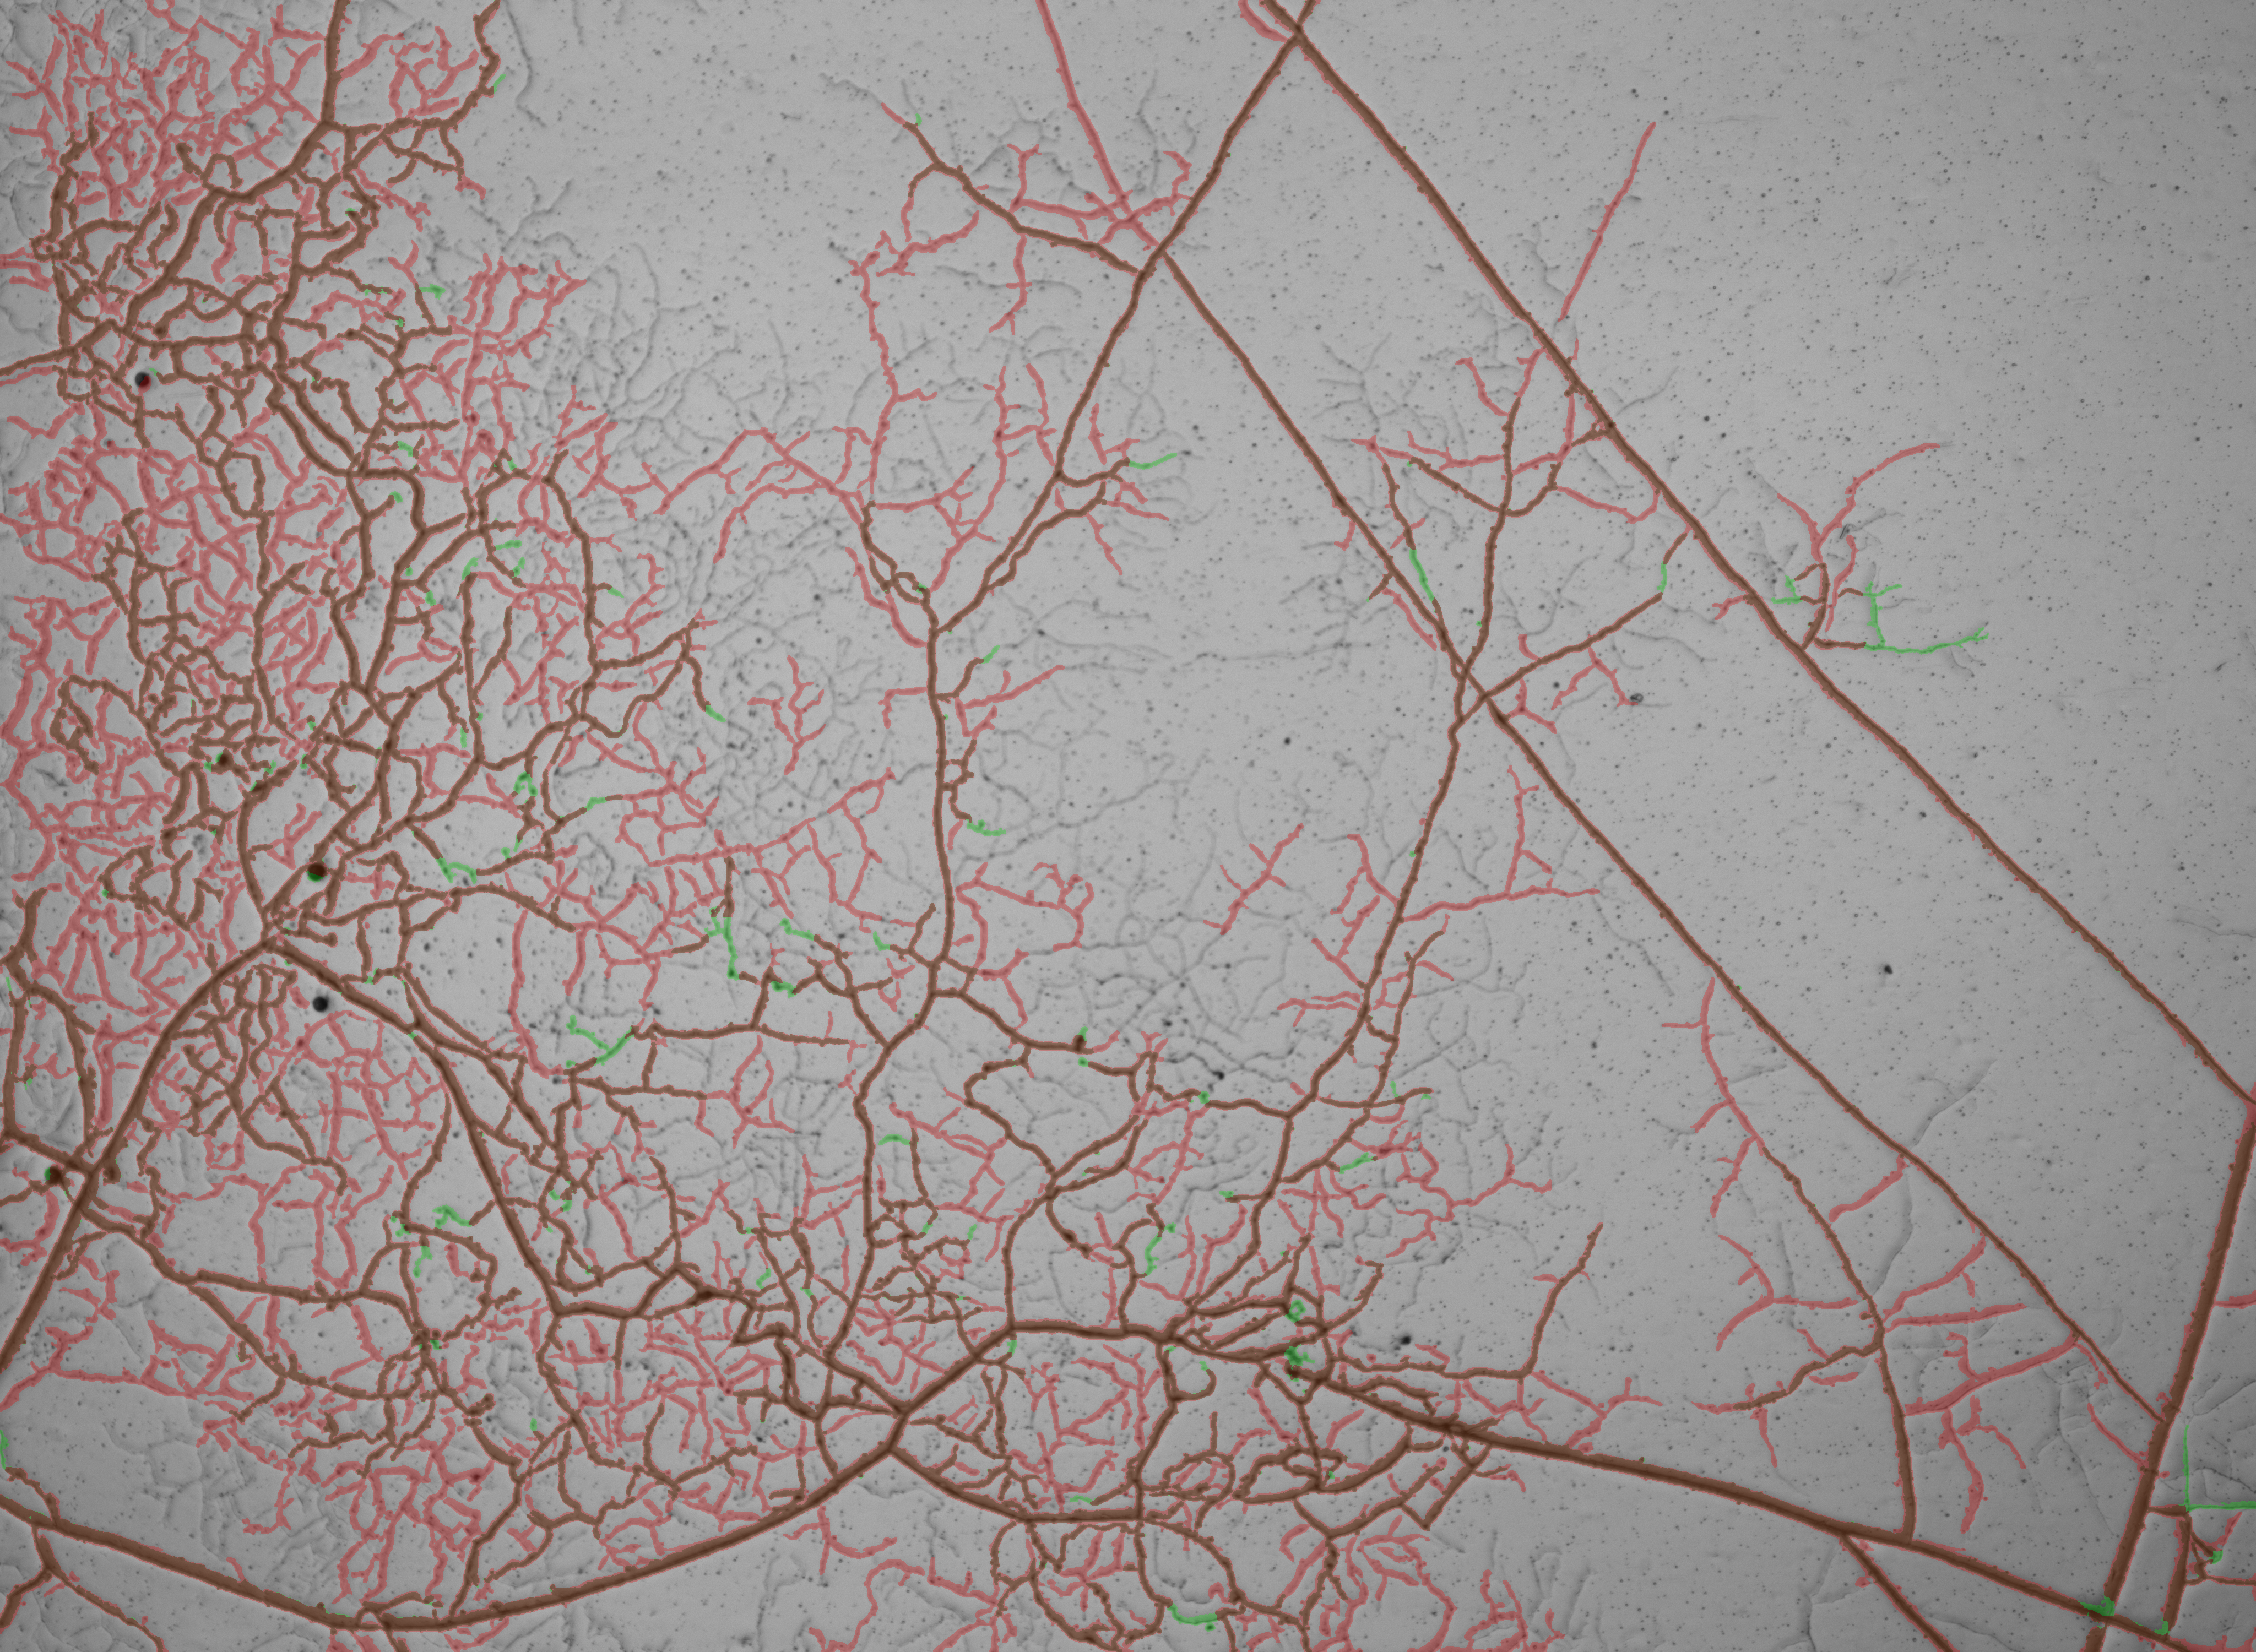
\includegraphics[width=0.9\textwidth]{suppfig/symbiotic-hard-comparison.png}
% TRIAGED 2 Oct: dense network with a segmentation overlay: an older segmentation check. Suggest replace with the current pipeline SI figures (S_segmenter, S_graph_repair) or drop (transport_paper#129).
\caption{\textbf{TODO: Symbiotic hard comparison.}
TODO caption.}
% \label{fig:symbiotic_comparison}
\end{figure}
